\documentclass[tikz,border=3mm]{standalone}
\usepackage{pgfplots}
\begin{document}
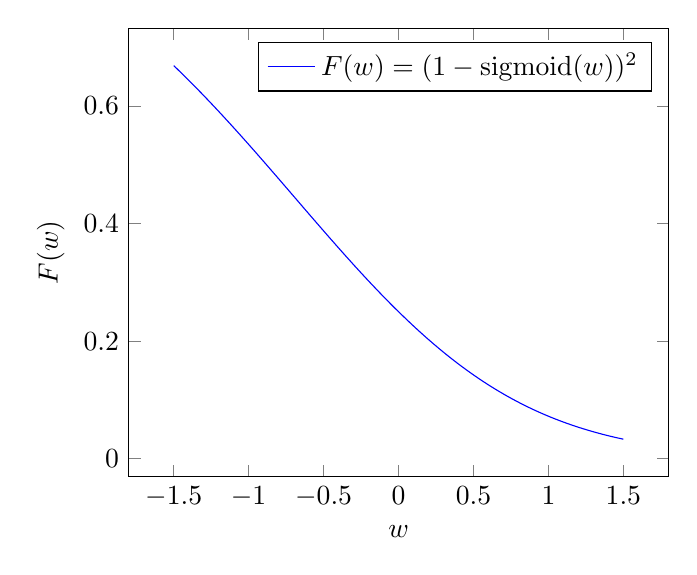
\begin{tikzpicture}
    \begin{axis}[
    xlabel=$w$,
    ylabel=$F(w)$,
    domain=-1.5:1.5,samples=400,
    legend pos=  north east,]
        \addplot+[mark=none] {(1-1/(1+exp(-x)))^2};
        \addlegendentry{$F(w)=(1-\mbox{sigmoid}(w))^2$};
    \end{axis}
\end{tikzpicture}

\end{document}